% \date{May 14, 2024}
% \author{Deralive}
% \title{华东师范大学软件学院实验报告模板}
% 注意事项:编译两次,以确保目录、页码完整显示

\def\allfiles{}

%————————————多文件编译————————————%
% \ifx\allfiles\undefined
% 	    \begin{document}
% \else
% \fi

% Content

% \ifx\allfiles\undefined
% 	    \end{document}
% 	\else
% 	\fi
%—————————————————————————————————%

\documentclass[14pt,a4paper,UTF8,twoside]{article}

\usepackage{amsmath}
\usepackage{graphicx}
\usepackage{geometry} 
\usepackage{ctex}
\usepackage{booktabs} % 表格库
\usepackage{titlesec} % 标题库
\usepackage{fancyhdr} % 页眉页脚库
\usepackage{lastpage} % 页码数库
\usepackage{listings} % 代码块包
\usepackage{xcolor}
\usepackage[hidelinks]{hyperref}
\usepackage{tikz}
\usepackage{tikz-qtree}
\usepackage{fontspec} % 允许设置字体
\usepackage{unicode-math} % 允许数学公式使用特定字体
\usepackage{mwe}
\usepackage{zhlipsum} % 中文乱数文本
\usepackage{amsmath}
\usepackage{xcolor}
\usepackage{float} % 浮动体环境
\usepackage{subcaption} % 子图包
\usepackage{biblatex}
\usepackage{array}
\usepackage{multirow}
\addbibresource{references.bib} % 指定你的.bib文件名称

\definecolor{mygreen}{rgb}{0,0.6,0}
\definecolor{mygray}{rgb}{0.5,0.5,0.5}
\definecolor{mymauve}{rgb}{0.58,0,0.82}

\date{} % 留空,以让编译时去除日期

%———————————————注意事项—————————————————%

% 1、如果编译显示失败,但没有错误信息,就是 filename.pdf 正在被占用
% 2、在文件夹中的终端使用 Windows > xelatex filename.tex 也可编译

%—————————————华东师范大学———————————————%

% 论文制作时须加页眉,页眉从中文摘要开始至论文末
% 偶数页码内容为:华东师范大学硕士学位论文,奇数页码内容为学位论文题目

%————————定义 \section 的标题样式————————%

% 注意:\chapter 等命令,内部使用的是 \thispagestyle{plain} 的排版格式
% 若需要自己加上页眉,实际是在用 \thispagestyle{fancy} 的排版格式
% 加上下面这一段指令,就能够让 \section 也使用 fancy 的排版格式
% 本质就是让目录、第一页也能够显示页眉、页脚

\fancypagestyle{plain}{
  \pagestyle{fancy}
}

\title{华东师范大学软件学院课程作业} % 模板
\titleformat{\section}
    {\normalfont\bfseries\Large} % 字体大小、字体系列(\bfseries 为加粗)
    {\thesection}{1em}{}

% 设置章节的中文格式
\renewcommand\thesection{\chinese{section} \hspace{0pt}}
\renewcommand\thesubsection{\arabic{subsection} \hspace{0pt}}
% \renewcommand\thesubsubsection{\alph{subsubsection} \hspace{0pt}} % 字母编号
% \hspace{0pt} 是为了确保在章节编号和章节题目之间不要有空格,使得排版更为美观
    
%—————————————页面基础设置———————————————%

\geometry{left=10mm, right=10mm, top=20mm, bottom=20mm}

%————————————设置页眉、页脚——————————————%

\pagestyle{fancy} % 设置 plain style 的属性

% 设置页眉

\fancyhead[RE]{\leftmark} % Right Even 偶数页右侧显示章名 \leftmark 最高级别章名
\fancyhead[LO]{\rightmark} % Left Odd 奇数页左侧显示节名 \rightmark 第二级别节名
\fancyhead[C]{华东师范大学软件学院课程作业} % Center 居中显示
\fancyhead[LE,RO]{~\thepage~} % 在偶数页的左侧,奇数页的右侧显示页码
\renewcommand{\headrulewidth}{1.2pt} % 页眉与正文之间的水平线粗细

% 设置页脚:在每页的右下脚以斜体显示书名

\fancyfoot[RO,RE]{\it Lab Report By \LaTeX} % 使用意大利斜体显示
\renewcommand{\footrulewidth}{0.5pt} % 页脚水平线宽度

% 设置页码:在底部居中显示页码

\pagestyle{fancy}
\fancyfoot[C]{\kaishu 第 \thepage 页 \ 共 \pageref{LastPage} 页} % LastPage 需要二次编译以获取总页数

%——————————————代码块设置———————————————%

\lstset {
    backgroundcolor=\color{white},   % choose the background color; you must add \usepackage{color} or \usepackage{xcolor}
    basicstyle=\footnotesize,        % the size of the fonts that are used for the code
    breakatwhitespace=false,         % sets if automatic breaks should only happen at whitespace
    breaklines=true,                 % sets automatic line breaking
    captionpos=bl,                   % sets the caption-position to bottom
    commentstyle=\color{mygreen},    % comment style
    deletekeywords={...},            % if you want to delete keywords from the given language
    escapeinside={\%*}{*},           % if you want to add LaTeX within your code
    extendedchars=true,              % lets you use non-ASCII characters; for 8-bits encodings only, does not work with UTF-8
    frame=single,                    % adds a frame around the code
    keepspaces=true,                 % keeps spaces in text, useful for keeping indentation of code (possibly needs columns=flexible)
    keywordstyle=\color{blue},       % keyword style
    % language=Python,               % the language of the code
    morekeywords={*,...},            % if you want to add more keywords to the set
    numbers=left,                    % where to put the line-numbers; possible values are (none, left, right)
    numbersep=5pt,                   % how far the line-numbers are from the code
    numberstyle=\tiny\color{mygray}, % the style that is used for the line-numbers
    rulecolor=\color{black},         % if not set, the frame-color may be changed on line-breaks within not-black text (e.g. comments (green here))
    showspaces=false,                % show spaces everywhere adding particular underscores; it overrides 'showstringspaces'
    showstringspaces=false,          % underline spaces within strings only
    showtabs=false,                  % show tabs within strings adding particular underscores
    stepnumber=1,                    % the step between two line-numbers. If it's 1, each line will be numbered
    stringstyle=\color{orange},      % string literal style
    tabsize=2,                       % sets default tabsize to 2 spaces
    % title=Python Code              % show the filename of files included with \lstinputlisting; also try caption instead of title
}

% 注释掉的部分用于后续插入代码,参数可调整,格式如下:

% 1、直接插入
% \begin{lstlisting}[language = ? , title = { ? } ]
%       Your code here.
% \end{lstlisting}

% 2、文件插入
% \lstinputlisting[language = C , title = ?.c] {filename.c}

%———————————————字体设置————————————————%

% \setCJKmainfont{SimSun} % 设置正文罗马族的 CJK 字体
% \renewcommand{\normalsize}{\fontsize{12pt}{15pt}\selectfont} % 设置正文字号
\linespread{1.2}

%——————————————————————————————————————%

%——————————————导言区结束,进入正文部分———————————————%

%——————————————————————————————————————%

\begin{document}

\maketitle

\begin{center} % \extracolsep{\fill} 拉伸到页面最大宽度前,保证居中显示

  \begin{tabular*}{\textwidth}{@{\extracolsep{\fill}} l  l  l }
    \hline
    课程名称:软件质量分析 &  年级:2023级本科  &  姓名:张梓卫 \\
    作业主题:总结软件可靠性定义 & 学号:10235101526 & 作业日期:2024/9/26 \\
    指导老师:陈仪香 & 组号: \\
    \hline
  \end{tabular*}

\end{center}

\tableofcontents % 目录也需要二次编译

\section{软件可靠性分析}

\subsection{定义}

按照GB/T11457-95-软件工程术语,软件可靠性的定义为:

(一:定量定义)在规定的条件(软件运行的软、硬环境、操作剖面:即软件运行的输入空间及其概率分布)下,
在规定的时间内软件不引起系统失效的概率。

其中:
\begin{itemize}
  \item 该概率是系统输入和系统使用的函数,也是软件中存在的缺陷的函数。
  \item 系统输入将确定是否运到已存在的缺陷。
  \item 输入空间:软件所有可能的输入值构成的空间。
  \item 操作剖面:系统使用条件的定义。
\end{itemize}

(二:定性定义)在规定的时间(执行时间、日历时间、时钟时间)周期内所述条件下程序执行所要求的功能的能力。

其中:
\begin{itemize}
  \item 执行时间:一个程序所用的实际时间或CPU时间(激励软件发生失效)【软件可靠性模型是针对执行时间建立的】
  \item 日历时间:编年时间,包括计算机可能未运行的时间。
  \item 时钟时间:程序执行开始到程序执行完毕所经过的钟表时间,该时间包括了其他程序运行的时间。
\end{itemize}

\section{软件失效机理}

\subsection{基础概念}

发生的失效数越多,或者发生失效的时间间隔越短,软件越不可靠。

\subsection{软件失效机理}

\subsubsection{失效的原因总结}

其中,软件失效分为四个可能的部分。

\begin{itemize}
  \item 错误(开发者):指开发人员在开发过程中出现的失误、疏忽和错误。
  \begin{itemize}
    \item 遗漏或误解软件需求规格说明中的用户需求
    \item 不正确的翻译或遗漏设计规格说明的需求
  \end{itemize}
  \item 缺陷(程序固有):代码中能引起一个或多个失效的错误的编码。
  \begin{itemize}
    \item 软件缺陷是程序固有的
    \item 软件文档中不正确的描述也称为缺陷
    \item 不正确的功能需求、遗漏的性能需求
  \end{itemize}
  \item 故障(运行时):是由于软件缺陷在运行时引起并产生的错误状态
  \begin{itemize}
    \item 不正确的数值等
    \item 数据在传输过程中产生的偏差
  \end{itemize}
  \item 失效(用户经历):程序的运行偏离了需求,是动态运行的结果。(遇到缺陷时)。
  \begin{itemize}
    \item 死机、错误的输出结果
    \item 超出规定时间的响应
  \end{itemize}
\end{itemize}

\subsection{失效的随机性}

存在随机性的原因:
\begin{itemize}
  \item 程序执行的条件不可预测
  \item 程序的使用千差万别
  \item 缺陷或错误在程序中的位置未知
\end{itemize}

\section{MTTF计算公式}

其中,TF指的是To Failure

\subsection{当不考虑软件失效情况}

\[
  \frac{1}{TFs} = \sum_{i=1}^{n} \frac{1}{TF_{i}}
\]

Example:

\begin{figure} [H]
  \centering
  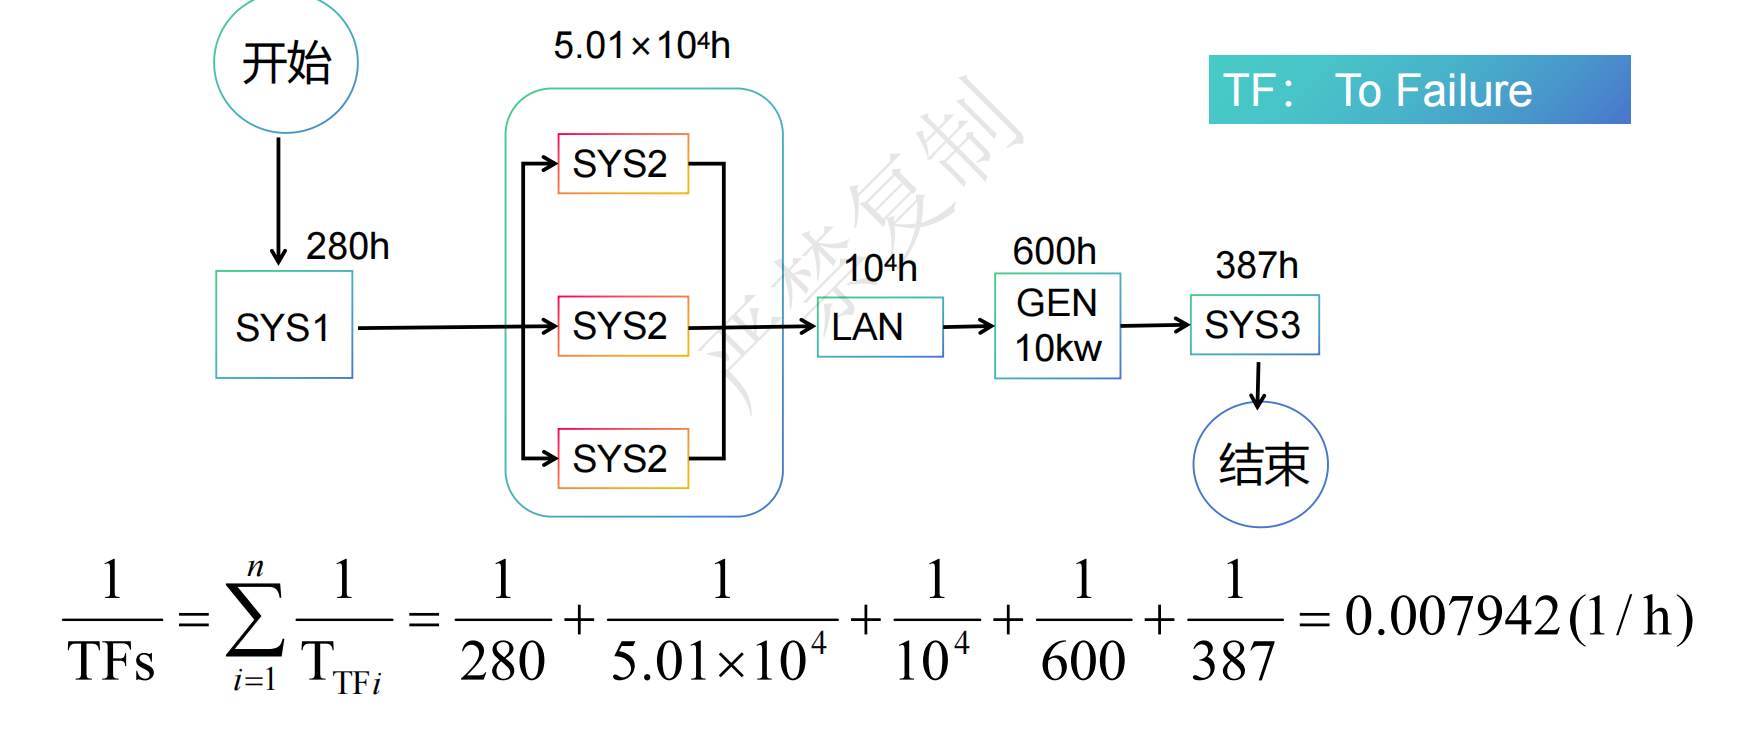
\includegraphics[width=0.6\textwidth]{img2/mttf.png}
  \label{fig:mttf}
\end{figure}

此时,\( TFs = \frac{1}{0.007942} = 125.9h \)

\subsection{考虑软件失效情况}

当考虑软件失效情况时(SYS2、SYS3初始失效率为2.52/h),则:

\begin{figure} [H]
  \centering
  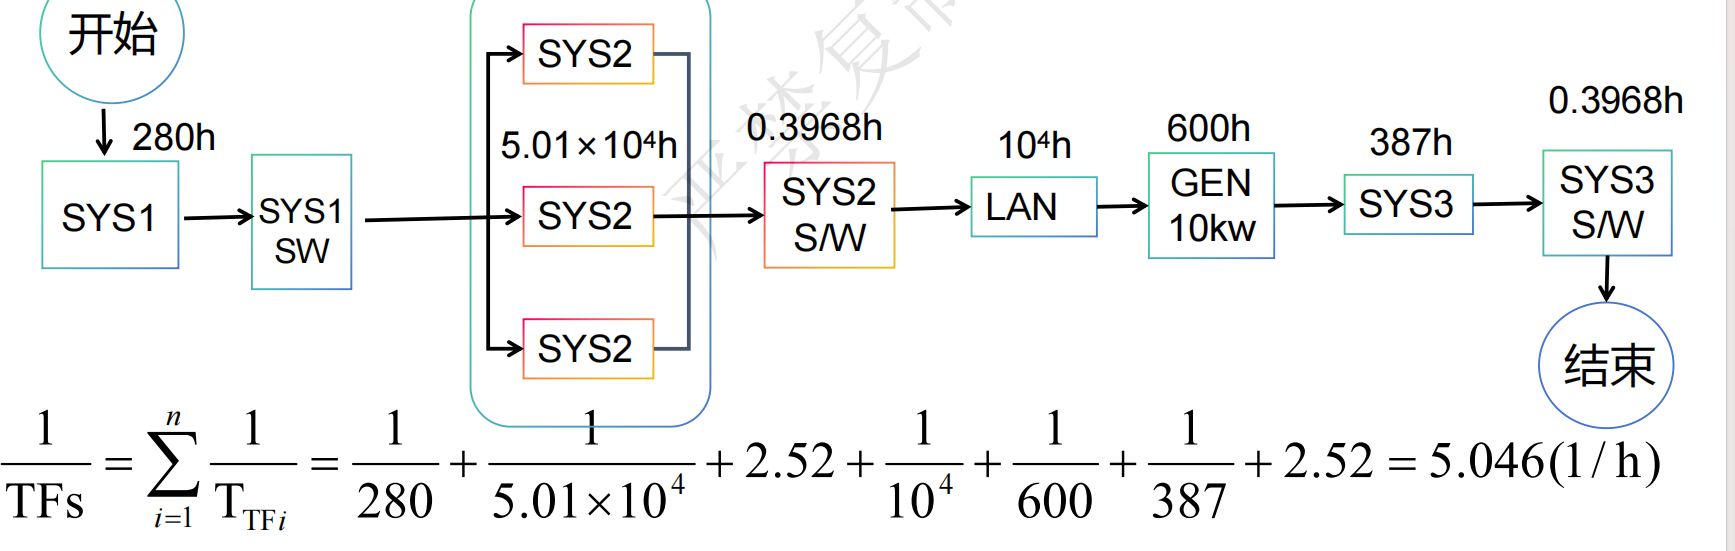
\includegraphics[width=0.6\textwidth]{img2/mttf2.png}
  \label{fig:mttf}
\end{figure}

此时,\( MTTF = \frac{1}{\frac{1}{TFs}} = 11.9 min \).

\section{软件的失效}

\subsection{定义失效严重等级}

应在软件需求说明中给出明确的项目特定的软件失效定义,因为软件可靠性是对失效行为特性的刻画,对于不同严重程度的失效用户常常有不同的要求。

Notice:

软件失效等级从对人员生命、成本、任务等方面考虑(分为1\~{}5级,1级最严重):

% \begin{itemize}
%   \item 1: 丧失生命或系统(>100,000\$)不能进行一项或多项关键操作
%   \item 2: 对完成的任务有影响(10,000~100,000\$)不能进行一项或多项重要操作
%   \item 3: 可采用绕过的措施,因而对过程只是极小的影响(达到了任务目标)(1,000~10,000\$)不能进行一项或多项操作,但有补救方法
%   \item 4: 对需求或标准有轻微的违反,用户在运行使用中看不见(<1000\$)一项或多项操作中的小缺陷
%   \item 5: 表面问题,对于将来的行动应予以注意或追踪,但不一定是现在需解决的问题
% \end{itemize}

\begin{tabular}{|c|m{3cm}|m{2.5cm}|m{3cm}|m{5cm}|}
  \hline
  \textbf{失效严重等级} & \textbf{生命影响定义} & \textbf{成本影响/美元} & \textbf{系统能力影响} & \textbf{可靠性要求示例(跨网络交易)} \\ \hline
  1 & 危及生命或系统 & >100,000 & 用户不能进行一项或多项关键操作 & 暂时的,有段损。一次跨网络的交易丢失导致了数据库损毁。失败率每1000次交易1次 \\ \hline
  2 & 对完成的任务有影响 & 10,000\~{}100,000 & 用户不能进行一项或多项重要操作 & 暂时的,无段损。无法读取一张非损坏的卡的磁条数据。成功率1/1000次交易 \\ \hline
  3 & 可采取统计措施,影响极小,任务可达成 & 1,000\~{}10,000 & 用户不能进行一项或多项操作,但有补救方法 & 永久的,无段损。系统对任何输入的卡都反应无效,软件必须更新来更正失效。失败率1/1000天 \\ \hline
  4 & 对需求或标准有轻微违反,运行中难以察觉 & <1,000 & 一项或多项操作中的小缺陷 & 无 \\ \hline
  5 & 表面问题,将影响行为应列为注意或追踪,但不一定需要当前解决 & 无 & 无 & 无 \\ \hline
\end{tabular}

\section{度量参数}

\subsection{失效率与失效强度}

\subsubsection{失效率}

失效率的定义和硬件可靠性中瞬时失效率的定义完全一致的,基于寿命的观点给出的。
它是一个条件概率密度。

失效率是指在 $t$ 时刻尚未发生失效的条件下,在 $t$ 时刻后单位时间内发生失效的概率。即:设 $\xi$ 为发生失效的时间,$Z(t)$ 为失效率,则有

\[
Z(t) = \lim_{\Delta t \to 0} \frac{P(t < \xi < t + \Delta t \mid \xi > t)}{\Delta t}
= \lim_{\Delta t \to 0} \frac{P(t < \xi < t + \Delta t)}{P(\xi > t) \cdot \Delta t}
= \lim_{\Delta t \to 0} \frac{R(t) - R(t + \Delta t)}{R(t) \cdot \Delta t}
\]

因此:

\[
Z(t) = -\frac{1}{R(t)} \cdot \frac{dR}{dt} = \frac{1}{R(t)} \cdot f(t)
\]


\subsubsection{失效强度}

失效强度则是基于随机过程定义的,是失效数均值的变化率。

假设软件在 $t$ 时刻发生的失效数是 $N(t)$,显然 $N(t)$ 是一个随机数,且随时间 $t$ 的变化而不同,即 $\{N(t), t > 0\}$ 是一个随机过程。设 $u(t)$ 为随机变量 $N(t)$ 的均值,即 $u(t) = E(N(t))$,则 $t$ 时刻的失效强度 $\lambda(t)$ 定义为:

\[
\lambda(t) = \frac{du(t)}{dt}
\]

\subsection{MTTF与MTBF}

\subsubsection{平均失效前时间MTTF}

MTTF 是指当前时间到下一次失效时间的均值。

\textbf{MTTF用于不可修复产品}

假设当前时间到下一次失效的时间为 $\xi$,$\xi$ 具有累计算率密度函数 $F(t) = P(\xi \leq t)$,即可靠度函数:

\[
R(t) = 1 - F(t) = P(\xi > t)
\]

则基于 MTTF 的软件可靠度 $T_{TF}$ 为:

\[
T_{TF} = \int_0^{\infty} R(t) dt
\]

\subsubsection{平均失效间隔时间MTBF}

定义与\textbf{平均失效前时间MTTF}相近,只需将 $\xi$ 转化为两次相邻失效时间间隔的均值即可。

\textbf{MTBF用于可修复产品}

\subsubsection{修复软件失效对软硬件的不一致性}

软件失效是可以修复的。但是,修复活动对失效特性的影响和硬件存在着很大的不同。

\begin{tabular}{|>{\raggedright\arraybackslash}p{8cm}|>{\raggedright\arraybackslash}p{8cm}|}
  \hline
  \textbf{理论} & \textbf{实际} \\
  \hline
  存在分析不可能得到的产品,如食品、电器 & 存在不能得到的文献,即实体档案都是可以得到的。 \\
  \hline
  文献后续进行完全框架,则失效率不变,原MTBF不变 & 文献后续框架生态化,原MTBF变化 \\
  \hline
  如果失效后不修而丢弃使用,修复对系统可靠性影响(与失效前之比),系统的失效率是变化的 & 失效后可以不修而丢弃,但与失效前相比,并不存在着避免修复。如果对原材料使用复杂且持续不变的话,材料失效率未必不变。这是因为回避不修,产品失效的可能与产品的使用频率有关,与产品的状况有关,而要满足一定的条件,确保回向导致失效的情况。 \\
  \hline
\end{tabular}

\subsection{缺陷密度与故障密度}

\subsubsection{缺陷密度(DD)}

软件缺陷的基本度量,用于设定产品质量目标,支持软件可靠性模型预测潜藏的软件缺陷。

公式如下:

\[
DD = \frac{D(\text{每个版本或模块规定严重性等级下的缺陷数})}{KSLOC(\text{代码的千行源代码数}(=\text{代码行数}/1000))}
\]

\subsubsection{故障密度}

按严重性分类将计算的故障密度与目标值比较来确定是否已经完成足够的测试。

公式如下:

\[
 FD = \frac{F(\text{导致严重性等级的失效的唯一故障数(相同故障记作一次)})}{KSLOC}
\]

\subsection{需求依从性}

量反映软件需求分析工作的度量。根据该度量可以确定在需求分析阶段,
软件需求规格说明中的需求不一致的比例,适用于\textbf{需求阶段}。

计算公式:


\textbf{数据元素}:
\begin{itemize}
    \item $I_R$ 表示由于不一致的需求而引起的错误比例;
    \item $N_R$ 表示由于不完整的需求而引起的错误比例;
    \item $M_R$ 表示由于曲解的需求而引起的错误比例。
\end{itemize}

\textbf{公式}:

\[
I_R = \left( \frac{N_1}{N_1 + N_2 + N_3} \right) \times 100\%
\]

\[
N_R = \left( \frac{N_2}{N_1 + N_2 + N_3} \right) \times 100\%
\]

\[
M_R = \left( \frac{N_3}{N_1 + N_2 + N_3} \right) \times 100\%
\]

\textbf{注释}:
\begin{itemize}
    \item $N_1$ 表示在一个版本或者模块中不一致的需求数。
    \item $N_2$ 表示在一个版本或者模块中不完整的需求数。
    \item $N_3$ 表示在一个版本或者模块中曲解的需求数。
    \item $N_1 + N_2 + N_3$ 是一个版本或者模块中不一致、不完整、易曲解的需求数之和。
\end{itemize}

\subsection{度量参数的选择}

\begin{itemize}
  \item (1)对失效发生频率要求较低的系统,可靠性参数可选失效率或
  失效强度,如操作系统、电话交换系统软件等。
  \item(2)对在规定时间内能无失效工作要求比较高的系统,可选可靠
  度作为软件可靠性参数,如火力控制系统软件等。
  \item(3)对使用比较稳定的软件,可选平均失效前时间/平均失效间隔
  时间作为软件可靠性参数,如通用软件包等。
\end{itemize}

\end{document}